% THIS IS SIGPROC-SP.TEX - VERSION 3.1
% WORKS WITH V3.2SP OF ACM_PROC_ARTICLE-SP.CLS
% APRIL 2009
%
% It is an example file showing how to use the 'acm_proc_article-sp.cls' V3.2SP
% LaTeX2e document class file for Conference Proceedings submissions.
% ----------------------------------------------------------------------------------------------------------------
% This .tex file (and associated .cls V3.2SP) *DOES NOT* produce:
%       1) The Permission Statement
%       2) The Conference (location) Info information
%       3) The Copyright Line with ACM data
%       4) Page numbering
% ---------------------------------------------------------------------------------------------------------------
% It is an example which *does* use the .bib file (from which the .bbl file
% is produced).
% REMEMBER HOWEVER: After having produced the .bbl file,
% and prior to final submission,
% you need to 'insert'  your .bbl file into your source .tex file so as to provide
% ONE 'self-contained' source file.
%
% Questions regarding SIGS should be sent to
% Adrienne Griscti ---> griscti@acm.org
%
% Questions/suggestions regarding the guidelines, .tex and .cls files, etc. to
% Gerald Murray ---> murray@hq.acm.org
%
% For tracking purposes - this is V3.1SP - APRIL 2009

\documentclass{acm_proc_article-sp}

\begin{document}

\title{Refugeesimulation}
\subtitle{Interactive Simulation WS15/16 \\ Project Proposal}
%
% You need the command \numberofauthors to handle the 'placement
% and alignment' of the authors beneath the title.
%
% For aesthetic reasons, we recommend 'three authors at a time'
% i.e. three 'name/affiliation blocks' be placed beneath the title.
%
% NOTE: You are NOT restricted in how many 'rows' of
% "name/affiliations" may appear. We just ask that you restrict
% the number of 'columns' to three.
%
% Because of the available 'opening page real-estate'
% we ask you to refrain from putting more than six authors
% (two rows with three columns) beneath the article title.
% More than six makes the first-page appear very cluttered indeed.
%
% Use the \alignauthor commands to handle the names
% and affiliations for an 'aesthetic maximum' of six authors.
% Add names, affiliations, addresses for
% the seventh etc. author(s) as the argument for the
% \additionalauthors command
% These 'additional authors' will be output/set for you
% without further effort on your part as the last section in
% the body of your article BEFORE References or any Appendices.

\numberofauthors{2} %  in this sample file, there are a *total*
% of EIGHT authors. SIX appear on the 'first-page' (for formatting
% reasons) and the remaining two appear in the \additionalauthors section.
%
\author{
% You can go ahead and credit any number of authors here,
% e.g. one 'row of three' or two rows (consisting of one row of three
% and a second row of one, two or three).
%
% The command \alignauthor (no curly braces needed) should
% precede each author name, affiliation/snail-mail address and
% e-mail address. Additionally, tag each line of
% affiliation/address with \affaddr, and tag the
% e-mail address with \email.
%
% 1st. author
\alignauthor
Markus Hofmann\\
       \affaddr{University of Augsburg}\\
       \email{markus.hofmann@student.uni-augsburg.de}
% 2nd. author
\alignauthor
Alexander Oks\\
       \affaddr{University of Augsburg}\\
       \email{alexander.oks@student.uni-\\augsburg.de}
}

\maketitle

\begin{abstract}
With our refugee-simulator we want to illustrate the flows of refugees in Europe according to decisions the user can take in some dialogues. In these he will get asked several questions about the current policy in Germany and policy towards Europe. It will all be displayed on an interactive map in 2D.

%which he get asked 
\end{abstract}

\section{Motivation}
For about a year more and more refugees escapes from their homeland to take refuge in Europe. They are coming from countries like Syria in which war or civil war prevails. But also countries without war are affected. For example refugees from the Balkan States are coming to Europe caused by the bad financial situation. Driven by poverty and/or their fear of life they all their few belongings behind to find a better place to improve the standard of living. At the moment many thousand of refugees are arriving Europe. Hence this subject is often discussed lately. With our simulation we want to inform the user about potential causes and possible approaches of huge refugee flows arriving Germany and adjoining countries. Therefore we want to create fictitious ``what-if''-scenarios, where the user can choose between many decisions about the refugee- and the general policy in their country to avoid a bigger crises.


%
% like Syria, where civil war
% The subject about refugees and the refugee-policy are often discussed lately. We want to inform the user about possible causes and potential approaches of refugee flows. Therefore

\section{Concept idea}
\label{concept idea}
The user assumes the role of a head of state. He/she has to make decisions concerning internal, foreign and economic policy. Those decisions have influence on the people of the users country  and on the other countries in the world which can lead to emerging refugee flows. The user has to decide what happens to the refugees which arrive at his country. 

\section{Project requirements}
In our simulation there should be four aspects that have to be involved.
\subsection{Science}
\subsubsection*{\textbf{General refugee policy}}
The user in his role as described in section \ref{concept idea} have to take many several decisions about the general refugee policy. For simplification only the decision-making for Germany and ruling from the European Parliament will take place. Therefore the president or similar will be confronted with questions like which people are allowed to come to their country. Thereby it has to be considered if they are coming from a country in which war or civil war is already being waged or are they coming from a so called ``save place'', where there is more or less poverty but no acts of war (see \ref{complexity}). Of course we can not foretell how many refugees will arrive Europe on the long term. Accordingly we will make use of current mean values of refugee flows. 

%In addition the user have to 

\subsubsection*{\textbf{Financial policy}}
For some calculations the financial policy of a country or a state is very important. Germany for example have to spend up to ten billion Euro for refugees, if they stay for one year \cite{finanzen}. Also at the moment Germany have to spend money for each refugee that will be send back to their country of origin \cite{auswanderung}. It is also the question where the money for the refugee relief should come from. Should we raise taxes or even levy new taxes. Thus it has to be considered that the people in a country will get upset if the taxes are too high. Therefore it could be helpful to involve the European Union to spread money they have raised from every country in the EU before. That money can be averaged of how many refugees they will receive. 

\subsubsection*{\textbf{Internal and foreign policy}}
Of course there is some internal and foreign policy that should be included. For example the large numbers of refugees that have to be divided within the country and/or all over Europe. For this purpose it had to be considered how many refugees a state or a country can handle at the same time. If the number of arriving refugees is too high, they will collapse and adjoining country have to receive additional refugees or should pay more money.


\subsection{Gamification}
\label{gamification}
In order to keep the user interested we define some main goals. One of the goals is to keep your citizens happy. The user also has to manage the finances of his/her country and manage the number of refugees. To accomplish those goals the user has to answer dialogues which occur on a regularly basis but also at some randomly generated special events. 
\subsection{Complexity}
\label{complexity}
One of the most important parts of this project is simulating how refugee flows emerge, where they come from how they behave. In order to simulate those points we want to classify the countries in the world by the attributes happiness, poverty, starvation and state of war. Based on those attributes Refugee flows emerge and start moving around the map.
\subsection{Aesthetics}
The aesthetical experience is based on a 2D-world map which shows countries and their basic attributes (\ref{complexity}). Furthermore we want to display refugee flows on the world map. They are represented visually  either  by dots, arrows or 2D sprites which move from one country to another on the world map. The user is interacting through dialogs which pop up as described in \ref{gamification}. A question and a set of answers are displayed inside of the up-popping windows. The attributes of countries and refugees are displayed inside of pop-up windows which appear when the user selects one of them with a mouse click.

\begin{figure}
\centering
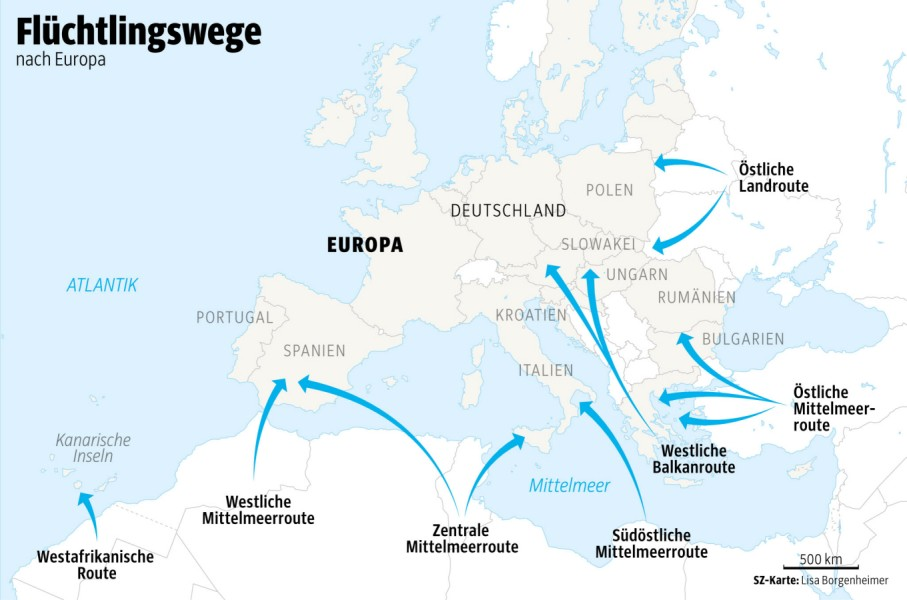
\epsfig{file=image.jpg, height=2.5in, width=3.3in}
\caption{Flows of refugees in Europe.}
\label{europe}
\end{figure}

\section{Concept user-experience}
The user experiences the simulation by navigating through the world map where he/she can see how the situation in the different countries is, where refugees emerge and where they go to. In the beginning the user gets some hints on where he /she can look things up. Clicking on a countriy for example opens a pop up window which shows the attributes of the country as described in (\ref{complexity}). Clicking on a refugee sprite shows further information about the refugee like where they come from, where they want to go to, how many of them are represented by this sprite and how likely they are to survive their journey. As time passes by more and more refugees emerge and try to come to the users` country. Now the user has to decide what to do. He/she could for example help or encourage other countries to accept more refugees or try to help states where conflicts are carried out or just improve the circumstances for refugees in his/her own country.
To keep the user challenged one also needs to get reelected by keeping his/her citizens happy. For interaction the user only uses a mouse. Possible interactions are navigating through the map by scrolling to the edges of the window, zooming in and out of the map with the mouse wheel, clicking on displayed items and answering dialogs through clicking on the specific answer.

\section{Timeline}
We want to collect information about the topic till mid of November and come up with a logic model that represents the collected information as good as possible till end of November. In that time we also want to familiarize ourselves with Unity3D. Until mid of  December we want to implement our model and build a prototype without focusing on the graphical aspect of the simulation.  Until beginning of January we want to include graphical components and make last adjustments to the simulation. In the last weeks left we want to focus on working on our project report and prepare our presentation.

\section{Conclusion}
This paper should provide a first insight on how we want to accomplish our project. Our main task at the moment is gaining knowledge of that difficult topic and collecting data. In the next step we do not only want to make that subject understandable for us but also design a model that makes that topic 	presentable by the computer. 

\bibliographystyle{abbrv}
\bibliography{bibo} 
%\balancecolumns
\end{document}
